\chapter{Implementation Documentation}
Detailed description of \textbf{database} and \textbf{backend components} and \textbf{functions}.  

\section{Database}
Full database schema of the application was already shown in previous chapter (\autoref{fig2.8:dbschemafull}). This chapter will introduce reader to detailed description of tables and their relations.  
\newline
Each database table is accompanied with example table preview, where: 
\begin{itemize}
  \item abbreviated column name: \underline{(a)},
  \item contracted/ommited info: \underline{...},
\end{itemize}
followed by full listing of attributes - datatypes, keys, etc.
\subsection{Object tables}
These are the tables in database modeling the object to satisfy the primary motivation defined as the (\autoref{fig1.2:uml}). These rows are then being converted to \textbf{Object} or \textbf{Array\textless Object\textgreater}  (Club, Cup, Page, PairPositionUser, Position, Post, RefereeRank, Region, StatPositionCnt, StatUserCnt, User) and returned to application page by appropriate Manager.
% \newline
\subsubsection*{sp\_posts}
\textbf{Post} is a static snippet of news for homepage of web application.
\newline
\underline{Table preview}
\begin{center}
  \begin{tabular}{||c c c c c c c||} 
  \hline
  id & timestamp & title & content & d\_flag(a) & auth\_id(a) & sign(a)  \\ [0.5ex] 
  \hline\hline
  1 & 2023-01-... & Running... & SwimmPair... & 1 & 21 & 0 \\ 
  \hline
  2 & 2023-03-...  & Updates & This web... & 1 & 21 & 0 \\ 
 \hline
  ... & ... & ... & ... & ... & ...  & ... \\ [0.5ex] 
  \hline
  \end{tabular}
\end{center}
\underline{Columns description}
\begin{enumerate}
  \setlength\itemsep{0em}
  \item \textbf{id$|$PK}, int(11) \textit{Auto Increment}
  \item \textbf{timestamp}, datetime \textit{NULL} \lbrack \textbf{CURRENT\_TIMESTAMP}\rbrack 
  \item \textbf{title}, text
  \item \textbf{content}, text
  \item \textbf{display\_flag}, tinyint(1)
  \item \textbf{author\_user\_id$|$FK}, int(11) \textit{NULL}
  \item \textbf{signature\_flag}, tinyint(1)
\end{enumerate}

\subsubsection*{sp\_users}
User is referee in the system. User is affiliated to Club has one of UserRights and one of tier from RefereeRank. His statistics are presented via StatUserCnt in public sites via PositionsManager.
\newline
\underline{Table preview}
\begin{center}
  \begin{tabular}{||c c c c c c c||} 
  \hline
  id & first\_name & last\_name & email & password & hash & ... \\ [0.5ex] 
  \hline\hline
  1 & Lukáš & Kousal & lukas@swim.cz & -PASS- & -HASH- & ... \\ 
  \hline
  ... & ... & ... & ... & ... & ... & ... \\
  \hline
  N & ... & ... & ... & ... & ... & ... \\ 
  \hline
 \end{tabular}
 \end{center}
 \underline{Columns description}
 \begin{enumerate}
   \setlength\itemsep{0em}
   \item \textbf{id$|$PK}, int(11) \textit{Auto Increment}
   \item \textbf{first\_name}, varchar(50)
   \item \textbf{last\_name}, varchar(50)
   \item \textbf{email}, varchar(100) //unique identifier
   \item \textbf{password}, varchar(100)
   \item \textbf{hash}, varchar(32)
   \item \textbf{active\_flag}, tinyint(1) \lbrack \textbf{0}\rbrack 
   \item \textbf{approved\_flag}, tinyint(1) \lbrack \textbf{0}\rbrack 
   \item \textbf{rights}, tinyint(1)
   \item \textbf{referee\_rank\_id$|$FK}, int(11)
   \item \textbf{affiliation\_club\_id$|$FK}, int(11)
\end{enumerate}

\subsubsection*{sp\_clubs}
Club is an administrative unit of swimming club grouping bunch of users. One User is ClubManager/1 from UserRights, the rest is Referee/0. It can organize.
\newline
\underline{Table preview}
\begin{center}
 \begin{tabular}{||c c c c c||} 
 \hline
 id & name & abbrev(a) & club\_id & img \\ [0.5ex] 
 \hline\hline
 1 & Klub plaveckých sportů Vyškov & KPSVy & 614 & vyskov.jpg \\  
 \hline
 ... & ... & ... & ... & ... \\ [0.5ex]
\hline
 14 & TJ Rožnov pod Radhoštěm & TJRo & 0 & roznov.jpg \\
 \hline
\end{tabular}
\end{center}
\underline{Columns description}
\begin{enumerate}
  \setlength\itemsep{0em}
  \item \textbf{id$|$PK}, int(11) \textit{Auto Increment}
  \item \textbf{name}, varchar(80)
  \item \textbf{abbreviation}, text
  \item \textbf{code} int(11) \textit{NULL}
  \item \textbf{img}, text \textit{NULL}
  \item \textbf{affiliation\_region\_id$|$FK}, int(11)
\end{enumerate}

\subsubsection*{sp\_cups}
Cups are stored in this table.
\newline
\underline{Table preview}
\begin{center}
 \begin{tabular}{||c c c c c c||} 
 \hline
 id & t\_st(a) & t\_e(a) & name & desc(a) & org\_c\_id(a) \\ [0.5ex] 
 \hline\hline
 1 & 2023-... & 2023-...& GJW Cup I. & Cup organized by ... & 2 \\ 
 \hline
 ... & ... & ... & ...&... & ...  \\ [0.5ex] 
 \hline
\end{tabular}
\end{center}
\underline{Columns description}
\begin{enumerate}
  \setlength\itemsep{0em}
  \item \textbf{id$|$PK}, int(11) \textit{Auto Increment}
  \item \textbf{time\_start}, date
  \item \textbf{time\_end}, date
  \item \textbf{name}, text
  \item \textbf{description}, text
  \item \textbf{organizer\_club\_id$|$FK}, int(11)
\end{enumerate}


\subsubsection*{sp\_positions}
Position is object representing task for Cup that has to be performed by User. It has internal id based on which it is wired through the system internally.
\newline
\underline{Table preview}
\begin{center}
 \begin{tabular}{||c c||} 
 \hline
 id & name  \\ [0.5ex] 
 \hline\hline
 1 & Vrchní rozhodčí \\ 
 \hline
 ... & ...  \\ [0.5ex]
\hline
 19 & Ostatní  \\
 \hline
\end{tabular}
\end{center}
\underline{Columns description}
\begin{enumerate}
  \setlength\itemsep{0em}
  \item \textbf{id$|$PK}, int(11), \textit{Auto Increment}
  \item \textbf{name}, varchar(45)
\end{enumerate}

\subsection{Relation tables}
Relation tables hold the most important information stored in the SwimmPair system - the \textbf{pairings} and \textbf{data for underlying statistics}. Both availability for cups and pairings to positions are represented here.
\subsubsection*{sp\_user\_cup\_availability}
This table stores relationships between referees/\underline{users} and \underline{cups} called availability. Referees are signed up by their team manager or themselves as available for the cup. In case of sudden inability to participate, the attendance\_flag is switched to 0 in case the user is already assigned to some position. In that case the administrator is going to see the user in red box.
\newline
\underline{Table preview}
\begin{center}
 \begin{tabular}{||c c c c||} 
 \hline
 id & cup\_id & user\_id & attendance\_flag  \\ [0.5ex] 
 \hline\hline
 1 & 3 & 21 & 1 \\ 
 \hline
 2 & 3 & 1 & 1 \\ 
 \hline
 7 & 3 & 19 & 0 \\ 
 \hline
 ... & ... & ... & ...  \\ [0.5ex] 
 \hline
\end{tabular}
\end{center}
\underline{Columns description}
\begin{enumerate}
  \setlength\itemsep{0em}
  \item \textbf{id$|$PK}, int(11) \textit{Auto Increment}
  \item \textbf{cup\_id$|$FK}, int(11)
  \item \textbf{user\_id$|$FK}, int(11)
  \item \textbf{attendance\_flag}, tinyint(1) \lbrack \textbf{\textbf{1}}\rbrack 
\end{enumerate}

\subsubsection*{sp\_user\_position\_pairing}
This table stores pairing information about available referees/users on positions for each cup. This is the most time saving utility of the SwimmPair.
\newline
\underline{Table preview}
\begin{center}
 \begin{tabular}{||c c c c||} 
 \hline
 id & cup\_id & position\_id & user\_id  \\ [0.5ex] 
 \hline\hline
 46 & 5 & 5 & 21 \\ 
 \hline
 484 & 3 & 1 & 21 \\ 
 \hline
 485 & 3 & 1 & 22 \\ 
 \hline
 486 & 3 & 2 & 7 \\
 \hline
 487 & 3 & 3 & 15 \\
 \hline
 487 & 3 & 5 & 12 \\
 \hline
 487 & 3 & 7 & 14 \\
 \hline
 ... & ... & ... & ... \\ [0.5ex] 
 \hline
\end{tabular}
\end{center}
\underline{Columns description}
\begin{enumerate}
  \setlength\itemsep{0em}
  \item \textbf{id$|$PK}, bigint(20) \textit{Auto Increment}
  \item \textbf{cup\_id$|$FK}, int(11)
  \item \textbf{position\_id$|$FK}, int(11)
  \item \textbf{user\_id$|$FK}, int(11)
\end{enumerate}
\subsection{Content adjustment tables}
\subsubsection*{sp\_public\_stats\_config}
Configuration table of which positions in what order should be displayed in statistics on frontend. For frontend then LEFT-JOIN \textbf{position\_id} from table \textbf{sp\_positions} ON \textbf{id} and display \textbf{sp\_positions.name}.
\newline
\underline{Table preview}
\begin{center}
 \begin{tabular}{||c c||} 
 \hline
 id & position\_id  \\ [0.5ex] 
 \hline\hline
 148 & 1 \\ 
 \hline
 149 & 8  \\ 
 \hline
 150 & 2  \\ 
 \hline
 151 & 4  \\ 
 \hline
 152 & 6  \\  
 \hline
 \end{tabular}
\end{center}
\underline{Columns description}
\begin{enumerate}
  \setlength\itemsep{0em}
  \item \textbf{id$|$PK}, int(11) \textit{Auto Increment}
  \item \textbf{position\_id$|$FK}, int(11)
\end{enumerate}

\subsubsection*{sp\_pages}
\textbf{Page} is static website page with information in web application. It has some title and content.
\newline
\underline{Table preview}
\begin{center}
 \begin{tabular}{||c c c||} 
 \hline
 id & title & content \\ [0.5ex] 
 \hline\hline
 1 & Kontakty &  \textless h1\textgreater Title\textless /h1\textgreater  \textless p\textgreater Contact information +420...\textless /p\textgreater  \\

 \hline
\end{tabular}
\end{center}
\underline{Columns description}
\begin{enumerate}
  \setlength\itemsep{0em}
  \item \textbf{id$|$}, int(11) \textit{Auto Increment}
  \item \textbf{title}, text
  \item \textbf{content}, text
\end{enumerate}
\newpage
\section{Managers documentation}
\par These five managers work with objects and provide views and functions (i.e. joining more tables in varios ways to achieve all functionality). We're providing an overview of which API functions are calling which internal functions (plain, in cycle) and what are desired return values.  
\newline
\textbf{Documentation of model - classes and public functions is available \footnote{\url{http://docu.swimmpair.cz}}}.

\subsection{PostsManager.php}
PostsManager has API functions to handle Post object/s and delivers it through web application.
\begin{itemize}
  \setlength\itemsep{0em}
  \item \underline{Post} $\vert$ null $\leftarrow$ \textbf{GetPostById}(\$id)
  \newline    $\searrow$ \_CreatePostOrNullFromStatement(\$stmt)
  \newline    $\searrow$ \_CreatePostFromRow(\$row)
  \item \underline{Post[]} $\vert$ null $\leftarrow$ \textbf{FindLastNPosts}(\$N)
  \newline    $\searrow$ \_CreatePostsFromStatement(\$stmt)
  \newline    $\hookrightarrow$ \_CreatePostFromRow(\$row)
  \item \underline{true} $\vert$ false $\leftarrow$ \textbf{InsertNewPost}(\$title, \$content, \$d\_flag, \$auth\_id, \$sign)
  \item \underline{Post[]} $\vert$ false $\leftarrow$ \textbf{FindAllPostsOrderedByIdDesc}()
  \newline    $\searrow$ \_CreatePostsFromStatement(\$stmt)
  \newline    $\hookrightarrow$ \_CreatePostFromRow(\$row)
  \item \underline{true} $\vert$ false $\leftarrow$ \textbf{UpdatePost}(\$id, \$title, \$content, \$d\_flag, \$sign)
\end{itemize}

\subsection{UsersManager.php}
UsersManager has API functions to handle User object/s and delivers is through web application.
\begin{itemize}
  \setlength\itemsep{0em}
  \item \underline{User} $\vert$ null $\leftarrow$ \textbf{GetUserById}(\$id)
  \newline    $\searrow$ \_CreateUserOrNullFromStatement(\$stmt)
  \newline    $\searrow$ \_CreateUserFromRow(\$row)
  \item \underline{User[]} $\vert$ null $\leftarrow$ \textbf{FindAllActiveUsersOrderByLastNameAsc}()
  \newline    $\searrow$ \_CreateUsersFromStatement(\$stmt)
  \newline    $\hookrightarrow$ \_CreateUserFromRow (\$row)
  \item \underline{User[]} $\vert$ null $\leftarrow$ \textbf{FindAllInactiveUsersOrderByLastNameAsc}()
  \newline    $\searrow$ \_CreateUsersFromStatement(\$stmt)
  \newline    $\hookrightarrow$ \_CreateUserFromRow (\$row)
  \item \underline{User[]} $\vert$ null $\leftarrow$ \textbf{FindAllRegisteredTeamMembersForTheCup}(\$cupId, \$teamId)
  \newline    $\searrow$ \_CreateUsersFromStatement(\$stmt)
  \newline    $\hookrightarrow$ \_CreateUserFromRow (\$row)
  \item \underline{User[]} $\vert$ null $\leftarrow$ \textbf{FindAllTeamMembers}(\$teamId)
  \newline    $\searrow$ \_CreateUsersFromStatement(\$stmt)
  \newline    $\hookrightarrow$ \_CreateUserFromRow(\$row)
  \item \underline{User[]} $\vert$ null $\leftarrow$ \textbf{FindAllRegisteredUsersForTheCup}(\$cupId)
  \newline    $\searrow$ \_CreateUsersFromStatement(\$stmt)
  \newline    $\hookrightarrow$ \_CreateUserFromRow(\$row)
  \item \underline{User[]} $\vert$ null $\leftarrow$ \textbf{FindPairedUsersOnCupForPosition}(\$cupId, \$posId)
  \newline    $\searrow$ \_CreateUsersFromStatement(\$stmt)
  \newline    $\hookrightarrow$ \_CreateUserFromRow(\$row)
  \item \underline{string} $\vert$ null $\leftarrow$ \textbf{GetClubAbbreviationByAffiliationId}(\$id)
  \newline    $\searrow$ \_GetSingleResultFromStatement(\$stmt)
  \item \underline{string} $\vert$ null $\leftarrow$ \textbf{GetUserFullNameById}(\$id)
  \newline    $\searrow$ \_GetSingleResultFromTwoColsStatement(\$stmt)
  \item \underline{true} $\vert$ \underline{false} $\leftarrow$ \textbf{IsEmailPresentAlready}(\$email)
  \item \underline{true} $\vert$ false $\leftarrow$ \textbf{RegisterUserFromAdmin}(\$first\_name, \$last\_name,
  \newline    \$email, \$password, \$rights, \$klubaffil)
  \item \underline{true} $\vert$ false $\leftarrow$ \textbf{EmailNewPersonRegistered}(\$email,
  \newline    \$password)
  \item \underline{true} $\vert$ false $\leftarrow$ \textbf{SetApprovedForUser}(\$userId)
  %\item \underline{true} $\vert$ false $\leftarrow$ \textbf{UpdatePairing}(\$JSON) //cupId, user-pos JSON
\end{itemize}

\subsection{ClubsManager.php}
ClubsManager has API functions to handle Club object/s and delivers it through web application.
\begin{itemize}
  \setlength\itemsep{0em}
  \item \underline{Club} $\vert$ null $\leftarrow$ \textbf{GetClubById}(\$id)
  \newline    $\searrow$ \_CreateClubFromStatement(\$stmt)
  \newline    $\searrow$ \_CreateClubFromRow(\$row)
  \item \underline{Club[]} $\vert$ null $\leftarrow$ \textbf{FindAllClubs}()
  \newline    $\searrow$ \_CreateClubsFromStatement(\$stmt)
  \newline    $\hookrightarrow$ \_CreateClubFromRow(\$row)
\end{itemize}

\subsection{CupsManager.php}
CupsManager has API functions to handle Cup object/s and delivers it through web application.
\begin{itemize}
  \setlength\itemsep{0em}
  \item \underline{Cup[]} $\vert$ null $\leftarrow$ \textbf{FindAllUpcomingCupsEarliestFirst}()
  \newline    $\searrow$ \_CreateCupsFromStatement(\$stmt)
  \newline    $\hookrightarrow$ \_CreateCupFromRow(\$row)
  \item \underline{Cup[]} $\vert$ null $\leftarrow$ \textbf{FindAllPastCupsMostRecentFirst}()
  \newline    $\searrow$ \_CreateCupsFromStatement(\$stmt)
  \newline    $\hookrightarrow$ \_CreateCupFromRow(\$row)
  \item \underline{Cup} $\vert$ null  $\leftarrow$  \textbf{GetCupById}(\$id)
  \newline    $\searrow$ \_CreateCupOrNullFromStatement(\$stmt)
  \newline    $\searrow$ \_CreateCupFromRow(\$row)
  \item \underline{Pair[]} $\vert$ null $\leftarrow$  \textbf{FindPairingsForThisCup}(\$id)
  \newline    $\searrow$ \_CreatePairsFromStatement(\$stmt)
  \newline    $\hookrightarrow$ \_CreatePairFromRow(\$row)
  \item \underline{true} $\vert$ false $\leftarrow$  \textbf{InsertNewCup}(\$name, \$t\_st, \$t\_end, \$club, \$content)
  \item \underline{true} $\vert$ \underline{false} $\leftarrow$  \textbf{IsUserAvailableForTheCup}(\$userId, \$cupId)
\end{itemize}
Called together in XMLHttpRequest/\textbf{update\_availability.php} in transaction.  
  \begin{itemize}
  \item \underline{true} $\vert$ false $\leftarrow$ \textbf{DeleteOldAvailability}(\$cupId)
  \item \underline{true} $\vert$ false $\leftarrow$ \textbf{InsertNewAvailability}(\$cupId, \$userId, 1)
\end{itemize}
Called together in XMLHttpRequest/\textbf{update\_pairing.php} in transaction.  
  \begin{itemize}
  \item \underline{hash} $\vert$ null $\leftarrow$ \textbf{GetPairingHashForThisCup}(\$cupId)
  \newline    $\searrow$ \_GetSingleResultFromStatement(\$stmt)
  \item \underline{true} $\vert$ false $\leftarrow$ \textbf{DeleteOldPairing}(\$cupId)
  \item \underline{true} $\vert$ false $\leftarrow$ \textbf{InsertNewPairing}(\$cupId, \$posId, \$userId)
\end{itemize}

\subsection{PositionsManager.php}
PositionsManager has API functions to handle Position object/s and delivers it through web application.
\begin{itemize}
  \setlength\itemsep{0em}
  \item \underline{Position[]} $\vert$ null $\leftarrow$  \textbf{FindAllPositions}()
  \newline    $\searrow$ \_CreatePositionsFromStatement(\$stmt)
  \newline    $\hookrightarrow$ \_CreatePositionFromRow(\$row)
  \item \underline{string} $\vert$ null $\leftarrow$ \textbf{GetPositionNameById}(\$id)
  \newline    $\searrow$ \_GetSingleResultFromStatement(\$stmt)
\end{itemize}
\newpage
\section{Start file}
Start file is included the in beginning of each page. It serves for \textbf{connection to database},  \textbf{sanitization of input}, \textbf{definition of error handling} and most importantly \textbf{includes objects and managers} and subsequently \textbf{instantiates all managers} by passing reference to live database connection \textbf{\$mysqli} - their only constructor argument.
\begin{lstlisting}
/*Database credentials from environment*/
$host = getenv("DATABASE_HOST");
$user = getenv("DATABASE_USER");
$pass = getenv("DATABASE_PASS");
$db   = getenv("DATABASE_NAME");
/*Database connection and charset set*/
$mysqli = new mysqli($host, $user, $pass, $db) or die($mysqli->error);
$mysqli->set_charset('utf8');
/* Sanitization function */
function h($string)
{
    return htmlspecialchars($string);
}
/* Exception handling*/
error_reporting(E_ALL);
ini_set("display_errors", 1);
set_exception_handler(function () {
    echo "<h3 style=\"color: red;\">INVALID REQUEST</h3>";
    exit();
});
/* Objects and Managers inclusion*/
require __DIR__ . '/model/Sanitizer.php';
require __DIR__ . '/model/Auth.php';
require __DIR__ . '/model/Post.php';
require __DIR__ . '/model/PostsManager.php';
require __DIR__ . '/model/Page.php';
require __DIR__ . '/model/PagesManager.php';
require __DIR__ . '/model/StatUserCnt.php';
require __DIR__ . '/model/StatPositionCnt.php';
require __DIR__ . '/model/RefereeRank.php';
require __DIR__ . '/model/Region.php';
require __DIR__ . '/model/RegionsManager.php';
require __DIR__ . '/model/User.php';
require __DIR__ . '/model/UsersManager.php';
require __DIR__ . '/model/Cup.php';
require __DIR__ . '/model/PairPositionUser.php';
require __DIR__ . '/model/CupsManager.php';
require __DIR__ . '/model/Position.php';
require __DIR__ . '/model/PositionsManager.php';
require __DIR__ . '/model/Club.php';
require __DIR__ . '/model/ClubsManager.php';
/* Construction of Managers w/ reference to $mysqli */
$postsManager     = new PostsManager($mysqli);
$pagesManager     = new PagesManager($mysqli);
$usersManager     = new UsersManager($mysqli);
$clubsManager     = new ClubsManager($mysqli);
$cupsManager      = new CupsManager($mysqli);
$positionsManager = new PositionsManager($mysqli);
$regionsManager = new RegionsManager($mysqli);
\end{lstlisting}
\newpage
\section{Application structure - files defined}
\subsection*{User part of the system}
The system is running on Czech URLs for convinience reasons of browsing. English equivalents of route pages are attached in brackets to demonstrate what the pages do for non-czech speaker. There is no client side routing with traditional LAMP stack.  
\newline
\begin{forest}
  for tree={
    font=\ttfamily,
    grow'=0,
    child anchor=west,
    parent anchor=south,
    anchor=west,
    calign=first,
    edge path={
      \noexpand\path [draw, \forestoption{edge}]
      (!u.south west) +(7.5pt,0) |- node[fill,inner sep=1.25pt] {} (.child anchor)\forestoption{edge label};
    },
    before typesetting nodes={
      if n=1
        {insert before={[,phantom]}}
        {}
    },
    fit=band,
    before computing xy={l=15pt},
  }
[www.SwimmPair.cz/index.php
  [Zavody (Cups)
    [nadchazejici.php (upcoming.php)
      [zavod.php (cup.php)]
    ]
    [archiv.php (archive.php)
      [zavod.php (cup.php)] 
    ]
  ]
  [Rozhodci (Referees)
    [lide.php (users.php)
      [clovek.php (user.php)]
    ]
    [kluby.php (clubs.php)
      [klub.php (club.php)]
    ]
  ]
  [/pravidla/index.php (/rules/index.php)]
  [kontakty.php (contacts.php)]
  [/admin/index.php]
]
\end{forest}
\newpage
\subsection*{Admin part of the system} 
The administration has following structure. After going to /admin/index.php user gets logs in and goes to /administration/profile.php. Regarding user's rights (that are passed around along with other information in \textbf{SESSION}, retrievable like \textbf{\$SESSION\_['rights']}) one has following structure (\textbf{Administration}, \textbf{My Club}, \textbf{Me}). Each user has profile settings for reseting password and other stuff.  
\newline
\begin{forest}
  for tree={
    font=\ttfamily,
    grow'=0,
    child anchor=west,
    parent anchor=south,
    anchor=west,
    calign=first,
    edge path={
      \noexpand\path [draw, \forestoption{edge}]
      (!u.south west) +(7.5pt,0) |- node[fill,inner sep=1.25pt] {} (.child anchor)\forestoption{edge label};
    },
    before typesetting nodes={
      if n=1
        {insert before={[,phantom]}}
        {}
    },
    fit=band,
    before computing xy={l=15pt},
  }
[www.SwimmPair.cz/administration/profile.php
  [pridat\_aktualitu.php (add\_post.php)]
  [editovat\_aktuality.php (edit\_posts.php)
    [editovat\_aktualitu.php (edit\_post.php)]
  ]
  [nove\_registrovani.php (newly\_registered.php)]
  [rozhodci\_zavody.php (referees\_cups.php)
    [pairing.php (pairing.php)]
  ]
  [zaregistrovat\_uzivatele.php (register\_user.php)]
  [editovat\_profily.php (edit\_profiles.php)
    [editovat\_profil.php (edit\_profile.php)]
  ]
  [novy\_klub.php (add\_club.php)]
  [sprava\_klubu.php (edit\_clubs.php)
    [editovat\_klub.php (edit\_club.php)]
  ]
  [novy\_kraj.php (new\_region.php)]
  [sprava\_kraju.php (edit\_regions.php)
    [editovat\_kraj.php (edit\_region.php)]
  ]
  [konfigurace\_statistik.php (configure\_stats.php)]
  [editovat\_stranku.php (edit\_page.php)]
]
\end{forest}
\newline
\begin{forest}
  for tree={
    font=\ttfamily,
    grow'=0,
    child anchor=west,
    parent anchor=south,
    anchor=west,
    calign=first,
    edge path={
      \noexpand\path [draw, \forestoption{edge}]
      (!u.south west) +(7.5pt,0) |- node[fill,inner sep=1.25pt] {} (.child anchor)\forestoption{edge label};
    },
    before typesetting nodes={
      if n=1
        {insert before={[,phantom]}}
        {}
    },
    fit=band,
    before computing xy={l=15pt},
  }
[My Club
  [pridat\_zavod.php (add\_cup.php)]
  [prihlasit\_moje\_lidi.php (sign\_availability\_mates.php)
    [prihlasit\_moje\_lidi\_na.php (sign\_availability\_mates\_for.php)]
  ]
]
\end{forest}
\newline
\begin{forest}
  for tree={
    font=\ttfamily,
    grow'=0,
    child anchor=west,
    parent anchor=south,
    anchor=west,
    calign=first,
    edge path={
      \noexpand\path [draw, \forestoption{edge}]
      (!u.south west) +(7.5pt,0) |- node[fill,inner sep=1.25pt] {} (.child anchor)\forestoption{edge label};
    },
    before typesetting nodes={
      if n=1
        {insert before={[,phantom]}}
        {}
    },
    fit=band,
    before computing xy={l=15pt},
  }
[Me
  [sebe\_na\_zavod.php (myself\_for\_cup.php)
    [prihlasit\_se\_na.php (sign\_myself\_for.php)]
  ]
]
\end{forest}

\section{Templating of web and administration}
Each page layout of public website has common characteristics such as header, menu and footer. These sections are unified and included everywhere, therfore they are included everywhere. They are:
\begin{itemize}
    \item \textbf{HEADER},
    \item \textbf{MENU},
    \item Generated from result obtained by one or more manager calls. this section might be further updated via \textbf{XMLHttpRequest calls \& DOM modifications} of newly delivered data,
    \item \textbf{FOOTER}.
\end{itemize}
Homepage of administration panel /admin/profile.php after login gets assembled with regards to the rights of logged user. Ordering is following: Admin (2) \textgreater \: Club manager (1) \textgreater \: Swimming referee (0) and each user gets snippet of his and lower role snippets:
\begin{itemize}
    \item \textbf{SUPERUSER} menu snippet - \textbf{2},
    \item \textbf{CLUB MANAGER} menu snippet - \textbf{1},
    \item \textbf{SWIMMING REFEREE} menu snippet - \textbf{0}.
\end{itemize}
Access to different pages is then discriminated based on rights code on each page. \newline
\textbf{Rights check on each page in administration} 
\begin {lstlisting}
<?php
    require __DIR__ . '/../start.php';
    session_start();
    Auth::requireRole(UserRights::SuperUser);
    ...
?>    
...
\end{lstlisting}
\textbf{Static requireRole function on Auth class for access permission} 
\begin{lstlisting}
class Auth
{
	public static function requireRole($role)
	{
		if (!isset($_SESSION['rights']))
        {
			header('Location: /prihlaseni.php');
			exit();
		}
		//Rights sharply lower that user has, throw RuntimeException
		if ($_SESSION['rights'] < $role)
        {
			echo '<h1>Not enough rights</h1>';
			echo $_SESSION['rights'];
			echo $role;
			throw new RuntimeException();
		}
	}
}
\end{lstlisting}
\section{JavaScript functionality documentation}
Frontend functionality is implemented via Vanilla JavaScript. Majority of interactive stuff takes place on \textbf{public part} of the application. This section will give reader a glimpse into how things fork on the frontend.
\subsection*{Functions in js/SwimmPairFrontendJSLib.js}
Functions in this library were created to support Ajax calls and DOM operations for \textbf{public part} of our application. Functions have self-descriptive names, function parameter \textbf{this} means reference to the caller DOM element.  
\newline
Functions are general \& contain \textbf{XMLHttpRequest} and \textbf{DOM modification}:
\begin{itemize}
  \setlength\itemsep{0em}
  \item \textbf{GetPostAppendPost(PushLastId())}
  \newline    $\searrow$ ConstructNextPost(id, timestamp, title, content, author, signed)
  \item \textbf{ProcessClubForTheSeason(clubId, this)}
  \newline    $\searrow$ CommunicateClubStatsXhrAndUpdateTable(clubId, year)
  \newline    $\searrow$ UpdateClubStatsTable(returnedJSON)
  \item \textbf{ProcessPersonForTheSeason(userId, this)}
  \newline    $\searrow$ CommunicateUserStatsXhrAndUpdateTable(userId, year)
  \newline    $\searrow$ UpdateUserStatsTable(cnt, arr\_str)
\end{itemize}

\subsection*{Backend endpoints for XMLHttpRequests}
\begin{itemize}
    \item get\_post\_following.php, \textbf{GET args}: \textbf{id}
    \item get\_person\_statistics\_for\_the\_season.php, \textbf{GET args}: user\textunderscore \textbf{id}, \textbf{year}
    \item get\_club\_statistics\_for\_the\_season.php, \textbf{GET args}: club\textunderscore \textbf{id}, \textbf{year}
\end{itemize}

\subsection{Previous post - retrieve older post}
This button on the main page serves as a tool for loading next post. It has \textbf{onclick="GetPostAppendPost(PushLastId())"}. Both are JavaScript functions, \textbf{PushLastId()} detects id \textbf{\textless article class="post" id="X"... } of last article \textbf{class="post"} from DOM by querySelector and returns it. This value is then used as an argument of call \textbf{GetPostAppendPost(id)}. This function requests article by GET request \textbf{XMLHttpRequest/get\_following\_post.php?id=X}.  
The result can me:
\begin{itemize}
\item \textbf{null} - button is deleted since there are no other articles to pull from DB,
\item \textbf{post} - next article is constructed and appended from response.
\end{itemize}

\subsection{User statistics - year change}
All individual referees have seasons years picker when opened. Default season is the current season. Clicking different season visibily changes selected year and obtains appropriate statistics and updates the stats table. Clicking \textbf{\textless span onclick="ProcessPersonForTheSeason(userId, this)"... } calls inside \textbf{CommunicateStatsXhrAndPopulateStats(userId, year)} gets data from \textbf{XMLHttpRequest/call\_get\_person\_statistics\_for\_the\_season.php}\newline \textbf{?id=userId\&year=YYYY} and updates table. Also via \text{this} reference in call the button is marked as selected.  

\subsection{Club statistics - year change}
Club statistics are updated by clicking appropriate year that gets switched. Year onclick calls \textbf{ProcessClubForTheSeason(clubId, this)} which gets statistics by calling \textbf{CommunicateClubStatsXhrAndUpdateTable(clubId, year)}
\newline by calling \textbf{XMLHttpRequest/get\_club\_statistics\_for\_the\_season.php}
\newline \textbf{?id=clubId\&year=Year} and subsequently calling function modifying DOM 
\newline \textbf{UpdateClubStatsTable(returnedGetJSON)} which literally updates stats.

\subsection{Filtering referees}
Refiltering of referees is triggered by one of these (\autoref{fig3.1:filtering}) functions on events: 
\begin{itemize}
  \item \textbf{region changed} - onclick="RegionPickerChanged(this)", 
  \item \textbf{ref. rank changed} - onclick="RefereeRankPickerChanged(this)",
  \item \textbf{searchbar changed} - onkeyup="SearchBarChanged()".
\end{itemize}
\begin{figure}[h]	
	\centering
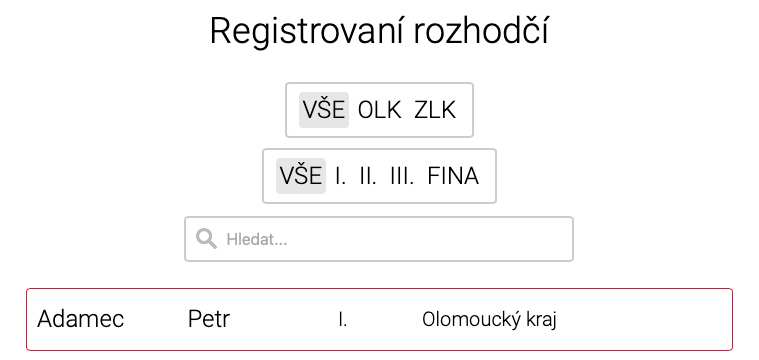
\includegraphics[scale=0.441]{img/filtering-preview.png}
%\underline{xyz}
\caption{Filtering of referees for statistics (requirements R3/S4).}
\label{fig3.1:filtering}
\end{figure}
\textbf{FilterQueriedReferees("kraje", "tridy", "inputTrida", "nopplfound")} is called every time one of 3 controls is changed. We then loop all users visible\&hidden and check if this one's \textbf{Region} IsOptionPermissible(raid, args[]) (region id), \textbf{Rank} IsOptionPermissible(rrid, args[]) (referee rank id) and then if one's \textbf{Name} IsNamePermissible(args[]) starts with searched piece of string. We then set one's element style to \textbf{style=""} and continue looping. If we fail one of these three conditions we know that referee does not fall under search conditions and set referee's element's style to \textbf{style="display:none"} - to make not visible in the listing.
\begin{lstlisting}
...  
  //Querying
  if (IsOptionPermissible(raid, krajeIDs)) {
      if (IsOptionPermissible(rrid, tridyIDs)) {
          if (IsNamePermissible(jmeno, first_name, last_name)) {
              articlePerson.setAttribute("style", "");
              empty = false;
              continue;
          }
      }
  }
  //Some Condition Fails - Not Permissible
  articlePerson.setAttribute("style", "display:none;");
}  
\end{lstlisting}
